\documentclass[border=10pt]{standalone}
\usepackage{tikz}

\begin{document}
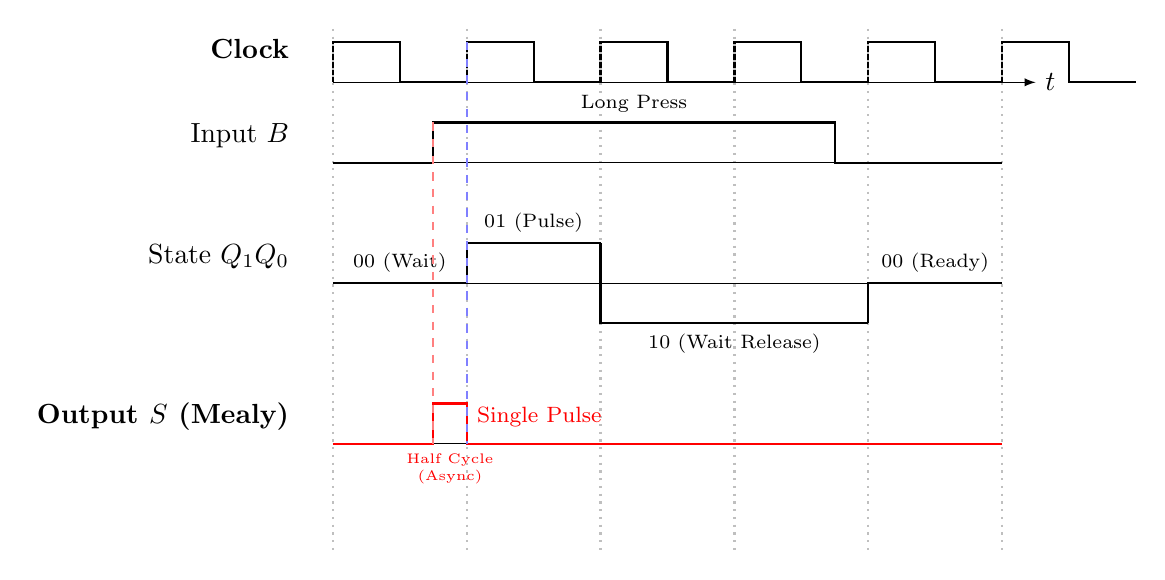
\begin{tikzpicture}[thick, >=latex, scale=0.85]
  % Define coordinates and heights
  \def\h{0.6}
  \def\w{1.5}
  \def\MAXT{10}
  
  % --- Clock ---
  \node[left, font=\bfseries] at (-0.5, 7.5) {Clock};
  \draw[thin, ->] (0, 7) -- (\MAXT+0.5, 7) node[right] {$t$};
  \foreach \i in {0,...,5} {
    \draw (\i*2, 7) -- ++(0, \h) -- ++(1, 0) -- ++(0, -\h) -- ++(1, 0);
    \draw[dotted, gray!50] (\i*2, 7.8) -- (\i*2, 0); % Vertical reference lines
  }
  
  % --- Input B ---
  \node[left] at (-0.5, 6.2) {Input $B$};
  \draw[thin] (0, 5.8) -- (\MAXT, 5.8);
  % B goes High at t=1.5 (Async), stays high until t=7.5
  \draw[thick] (0, 5.8) -- (1.5, 5.8) -- (1.5, 5.8+\h) -- (7.5, 5.8+\h) -- (7.5, 5.8) -- (\MAXT, 5.8);
  \node[above, font=\scriptsize] at (4.5, 5.8+\h) {Long Press};
  
  % --- State Q1 Q0 ---
  \node[left] at (-0.5, 4.4) {State $Q_1 Q_0$};
  \draw[thin] (0, 4.0) -- (\MAXT, 4.0);
  % Logic: 
  % 00 (Wait for B). Changes to 01 at next edge after B=1.
  % t=0-2: State 00. Edge t=2 captures B=1 -> 01.
  % t=2-4: State 01. Unconditional -> 10.
  % t=4-6: State 10. Wait for B=0. B=1 at edge t=6 -> Stay 10.
  % t=6-8. State 10. B=0 at edge t=8 -> 00.
  
  % State waveform (schematic representation of transitions)
  % 00
  \draw (0, 4.0) -- (2, 4.0); 
  \node[above, font=\scriptsize] at (1, 4.0) {00 (Wait)};
  
  % 2 -> 01
  \draw (2, 4.0) -- (2, 4.0+\h) -- (4, 4.0+\h);
  \node[above, font=\scriptsize] at (3, 4.0+\h) {01 (Pulse)};
  
  % 4 -> 10
  \draw (4, 4.0+\h) -- (4, 4.0) -- (4, 4.0-\h) -- (8, 4.0-\h);
  \node[below, font=\scriptsize] at (6, 4.0-\h) {10 (Wait Release)};
  
  % 8 -> 00
  \draw (8, 4.0-\h) -- (8, 4.0) -- (\MAXT, 4.0);
  \node[above, font=\scriptsize] at (9, 4.0) {00 (Ready)};
  
  
  % --- Output S (Mealy) ---
  \node[left, font=\bfseries] at (-0.5, 2.0) {Output $S$ (Mealy)};
  \draw[thin] (0, 1.6) -- (\MAXT, 1.6);
  
  % Logic: S = Q1' Q0' B (High only in 00 AND B=1)
  % t=0-1.5: State 00, B=0 -> S=0.
  % t=1.5-2: State 00, B=1 -> S=1 (Async Start!).
  % t=2: State becomes 01 -> S=0 (Sync Stop!).
  
  \draw[red, thick] (0, 1.6) -- (1.5, 1.6) -- (1.5, 1.6+\h) -- (2, 1.6+\h) -- (2, 1.6) -- (\MAXT, 1.6);
  
  \node[right, red, font=\footnotesize] at (2, 2.0) {Single Pulse};
  \node[below, red, font=\tiny, align=center] at (1.75, 1.6) {Half Cycle\\(Async)};

  % --- Guidelines ---
  \draw[dashed, red!50] (1.5, 6.4) -- (1.5, 1.6); % B rises -> S rises
  \draw[dashed, blue!50] (2, 7.6) -- (2, 1.6); % Clock edge -> State changes -> S falls

\end{tikzpicture}
\end{document}
